% Generated by Sphinx.
\def\sphinxdocclass{report}
\documentclass[letterpaper,10pt,english]{sphinxmanual}
\usepackage[utf8]{inputenc}
\DeclareUnicodeCharacter{00A0}{\nobreakspace}
\usepackage{cmap}
\usepackage[T1]{fontenc}
\usepackage{amsfonts}
\usepackage{babel}
\usepackage{times}
\usepackage[Bjarne]{fncychap}
\usepackage{longtable}
\usepackage{sphinx}
\usepackage{multirow}
\usepackage{eqparbox}


\addto\captionsenglish{\renewcommand{\figurename}{Fig. }}
\addto\captionsenglish{\renewcommand{\tablename}{Table }}
\SetupFloatingEnvironment{literal-block}{name=Listing }



\title{postqe Documentation}
\date{July 19, 2017}
\release{0.1}
\author{M. Palumbo, D. Brunato, P. D. Delugas}
\newcommand{\sphinxlogo}{}
\renewcommand{\releasename}{Release}
\setcounter{tocdepth}{2}
\makeindex

\makeatletter
\def\PYG@reset{\let\PYG@it=\relax \let\PYG@bf=\relax%
    \let\PYG@ul=\relax \let\PYG@tc=\relax%
    \let\PYG@bc=\relax \let\PYG@ff=\relax}
\def\PYG@tok#1{\csname PYG@tok@#1\endcsname}
\def\PYG@toks#1+{\ifx\relax#1\empty\else%
    \PYG@tok{#1}\expandafter\PYG@toks\fi}
\def\PYG@do#1{\PYG@bc{\PYG@tc{\PYG@ul{%
    \PYG@it{\PYG@bf{\PYG@ff{#1}}}}}}}
\def\PYG#1#2{\PYG@reset\PYG@toks#1+\relax+\PYG@do{#2}}

\expandafter\def\csname PYG@tok@gd\endcsname{\def\PYG@tc##1{\textcolor[rgb]{0.63,0.00,0.00}{##1}}}
\expandafter\def\csname PYG@tok@gu\endcsname{\let\PYG@bf=\textbf\def\PYG@tc##1{\textcolor[rgb]{0.50,0.00,0.50}{##1}}}
\expandafter\def\csname PYG@tok@gt\endcsname{\def\PYG@tc##1{\textcolor[rgb]{0.00,0.27,0.87}{##1}}}
\expandafter\def\csname PYG@tok@gs\endcsname{\let\PYG@bf=\textbf}
\expandafter\def\csname PYG@tok@gr\endcsname{\def\PYG@tc##1{\textcolor[rgb]{1.00,0.00,0.00}{##1}}}
\expandafter\def\csname PYG@tok@cm\endcsname{\let\PYG@it=\textit\def\PYG@tc##1{\textcolor[rgb]{0.25,0.50,0.56}{##1}}}
\expandafter\def\csname PYG@tok@vg\endcsname{\def\PYG@tc##1{\textcolor[rgb]{0.73,0.38,0.84}{##1}}}
\expandafter\def\csname PYG@tok@vi\endcsname{\def\PYG@tc##1{\textcolor[rgb]{0.73,0.38,0.84}{##1}}}
\expandafter\def\csname PYG@tok@mh\endcsname{\def\PYG@tc##1{\textcolor[rgb]{0.13,0.50,0.31}{##1}}}
\expandafter\def\csname PYG@tok@cs\endcsname{\def\PYG@tc##1{\textcolor[rgb]{0.25,0.50,0.56}{##1}}\def\PYG@bc##1{\setlength{\fboxsep}{0pt}\colorbox[rgb]{1.00,0.94,0.94}{\strut ##1}}}
\expandafter\def\csname PYG@tok@ge\endcsname{\let\PYG@it=\textit}
\expandafter\def\csname PYG@tok@vc\endcsname{\def\PYG@tc##1{\textcolor[rgb]{0.73,0.38,0.84}{##1}}}
\expandafter\def\csname PYG@tok@il\endcsname{\def\PYG@tc##1{\textcolor[rgb]{0.13,0.50,0.31}{##1}}}
\expandafter\def\csname PYG@tok@go\endcsname{\def\PYG@tc##1{\textcolor[rgb]{0.20,0.20,0.20}{##1}}}
\expandafter\def\csname PYG@tok@cp\endcsname{\def\PYG@tc##1{\textcolor[rgb]{0.00,0.44,0.13}{##1}}}
\expandafter\def\csname PYG@tok@gi\endcsname{\def\PYG@tc##1{\textcolor[rgb]{0.00,0.63,0.00}{##1}}}
\expandafter\def\csname PYG@tok@gh\endcsname{\let\PYG@bf=\textbf\def\PYG@tc##1{\textcolor[rgb]{0.00,0.00,0.50}{##1}}}
\expandafter\def\csname PYG@tok@ni\endcsname{\let\PYG@bf=\textbf\def\PYG@tc##1{\textcolor[rgb]{0.84,0.33,0.22}{##1}}}
\expandafter\def\csname PYG@tok@nl\endcsname{\let\PYG@bf=\textbf\def\PYG@tc##1{\textcolor[rgb]{0.00,0.13,0.44}{##1}}}
\expandafter\def\csname PYG@tok@nn\endcsname{\let\PYG@bf=\textbf\def\PYG@tc##1{\textcolor[rgb]{0.05,0.52,0.71}{##1}}}
\expandafter\def\csname PYG@tok@no\endcsname{\def\PYG@tc##1{\textcolor[rgb]{0.38,0.68,0.84}{##1}}}
\expandafter\def\csname PYG@tok@na\endcsname{\def\PYG@tc##1{\textcolor[rgb]{0.25,0.44,0.63}{##1}}}
\expandafter\def\csname PYG@tok@nb\endcsname{\def\PYG@tc##1{\textcolor[rgb]{0.00,0.44,0.13}{##1}}}
\expandafter\def\csname PYG@tok@nc\endcsname{\let\PYG@bf=\textbf\def\PYG@tc##1{\textcolor[rgb]{0.05,0.52,0.71}{##1}}}
\expandafter\def\csname PYG@tok@nd\endcsname{\let\PYG@bf=\textbf\def\PYG@tc##1{\textcolor[rgb]{0.33,0.33,0.33}{##1}}}
\expandafter\def\csname PYG@tok@ne\endcsname{\def\PYG@tc##1{\textcolor[rgb]{0.00,0.44,0.13}{##1}}}
\expandafter\def\csname PYG@tok@nf\endcsname{\def\PYG@tc##1{\textcolor[rgb]{0.02,0.16,0.49}{##1}}}
\expandafter\def\csname PYG@tok@si\endcsname{\let\PYG@it=\textit\def\PYG@tc##1{\textcolor[rgb]{0.44,0.63,0.82}{##1}}}
\expandafter\def\csname PYG@tok@s2\endcsname{\def\PYG@tc##1{\textcolor[rgb]{0.25,0.44,0.63}{##1}}}
\expandafter\def\csname PYG@tok@nt\endcsname{\let\PYG@bf=\textbf\def\PYG@tc##1{\textcolor[rgb]{0.02,0.16,0.45}{##1}}}
\expandafter\def\csname PYG@tok@nv\endcsname{\def\PYG@tc##1{\textcolor[rgb]{0.73,0.38,0.84}{##1}}}
\expandafter\def\csname PYG@tok@s1\endcsname{\def\PYG@tc##1{\textcolor[rgb]{0.25,0.44,0.63}{##1}}}
\expandafter\def\csname PYG@tok@ch\endcsname{\let\PYG@it=\textit\def\PYG@tc##1{\textcolor[rgb]{0.25,0.50,0.56}{##1}}}
\expandafter\def\csname PYG@tok@m\endcsname{\def\PYG@tc##1{\textcolor[rgb]{0.13,0.50,0.31}{##1}}}
\expandafter\def\csname PYG@tok@gp\endcsname{\let\PYG@bf=\textbf\def\PYG@tc##1{\textcolor[rgb]{0.78,0.36,0.04}{##1}}}
\expandafter\def\csname PYG@tok@sh\endcsname{\def\PYG@tc##1{\textcolor[rgb]{0.25,0.44,0.63}{##1}}}
\expandafter\def\csname PYG@tok@ow\endcsname{\let\PYG@bf=\textbf\def\PYG@tc##1{\textcolor[rgb]{0.00,0.44,0.13}{##1}}}
\expandafter\def\csname PYG@tok@sx\endcsname{\def\PYG@tc##1{\textcolor[rgb]{0.78,0.36,0.04}{##1}}}
\expandafter\def\csname PYG@tok@bp\endcsname{\def\PYG@tc##1{\textcolor[rgb]{0.00,0.44,0.13}{##1}}}
\expandafter\def\csname PYG@tok@c1\endcsname{\let\PYG@it=\textit\def\PYG@tc##1{\textcolor[rgb]{0.25,0.50,0.56}{##1}}}
\expandafter\def\csname PYG@tok@o\endcsname{\def\PYG@tc##1{\textcolor[rgb]{0.40,0.40,0.40}{##1}}}
\expandafter\def\csname PYG@tok@kc\endcsname{\let\PYG@bf=\textbf\def\PYG@tc##1{\textcolor[rgb]{0.00,0.44,0.13}{##1}}}
\expandafter\def\csname PYG@tok@c\endcsname{\let\PYG@it=\textit\def\PYG@tc##1{\textcolor[rgb]{0.25,0.50,0.56}{##1}}}
\expandafter\def\csname PYG@tok@mf\endcsname{\def\PYG@tc##1{\textcolor[rgb]{0.13,0.50,0.31}{##1}}}
\expandafter\def\csname PYG@tok@err\endcsname{\def\PYG@bc##1{\setlength{\fboxsep}{0pt}\fcolorbox[rgb]{1.00,0.00,0.00}{1,1,1}{\strut ##1}}}
\expandafter\def\csname PYG@tok@mb\endcsname{\def\PYG@tc##1{\textcolor[rgb]{0.13,0.50,0.31}{##1}}}
\expandafter\def\csname PYG@tok@ss\endcsname{\def\PYG@tc##1{\textcolor[rgb]{0.32,0.47,0.09}{##1}}}
\expandafter\def\csname PYG@tok@sr\endcsname{\def\PYG@tc##1{\textcolor[rgb]{0.14,0.33,0.53}{##1}}}
\expandafter\def\csname PYG@tok@mo\endcsname{\def\PYG@tc##1{\textcolor[rgb]{0.13,0.50,0.31}{##1}}}
\expandafter\def\csname PYG@tok@kd\endcsname{\let\PYG@bf=\textbf\def\PYG@tc##1{\textcolor[rgb]{0.00,0.44,0.13}{##1}}}
\expandafter\def\csname PYG@tok@mi\endcsname{\def\PYG@tc##1{\textcolor[rgb]{0.13,0.50,0.31}{##1}}}
\expandafter\def\csname PYG@tok@kn\endcsname{\let\PYG@bf=\textbf\def\PYG@tc##1{\textcolor[rgb]{0.00,0.44,0.13}{##1}}}
\expandafter\def\csname PYG@tok@cpf\endcsname{\let\PYG@it=\textit\def\PYG@tc##1{\textcolor[rgb]{0.25,0.50,0.56}{##1}}}
\expandafter\def\csname PYG@tok@kr\endcsname{\let\PYG@bf=\textbf\def\PYG@tc##1{\textcolor[rgb]{0.00,0.44,0.13}{##1}}}
\expandafter\def\csname PYG@tok@s\endcsname{\def\PYG@tc##1{\textcolor[rgb]{0.25,0.44,0.63}{##1}}}
\expandafter\def\csname PYG@tok@kp\endcsname{\def\PYG@tc##1{\textcolor[rgb]{0.00,0.44,0.13}{##1}}}
\expandafter\def\csname PYG@tok@w\endcsname{\def\PYG@tc##1{\textcolor[rgb]{0.73,0.73,0.73}{##1}}}
\expandafter\def\csname PYG@tok@kt\endcsname{\def\PYG@tc##1{\textcolor[rgb]{0.56,0.13,0.00}{##1}}}
\expandafter\def\csname PYG@tok@sc\endcsname{\def\PYG@tc##1{\textcolor[rgb]{0.25,0.44,0.63}{##1}}}
\expandafter\def\csname PYG@tok@sb\endcsname{\def\PYG@tc##1{\textcolor[rgb]{0.25,0.44,0.63}{##1}}}
\expandafter\def\csname PYG@tok@k\endcsname{\let\PYG@bf=\textbf\def\PYG@tc##1{\textcolor[rgb]{0.00,0.44,0.13}{##1}}}
\expandafter\def\csname PYG@tok@se\endcsname{\let\PYG@bf=\textbf\def\PYG@tc##1{\textcolor[rgb]{0.25,0.44,0.63}{##1}}}
\expandafter\def\csname PYG@tok@sd\endcsname{\let\PYG@it=\textit\def\PYG@tc##1{\textcolor[rgb]{0.25,0.44,0.63}{##1}}}

\def\PYGZbs{\char`\\}
\def\PYGZus{\char`\_}
\def\PYGZob{\char`\{}
\def\PYGZcb{\char`\}}
\def\PYGZca{\char`\^}
\def\PYGZam{\char`\&}
\def\PYGZlt{\char`\<}
\def\PYGZgt{\char`\>}
\def\PYGZsh{\char`\#}
\def\PYGZpc{\char`\%}
\def\PYGZdl{\char`\$}
\def\PYGZhy{\char`\-}
\def\PYGZsq{\char`\'}
\def\PYGZdq{\char`\"}
\def\PYGZti{\char`\~}
% for compatibility with earlier versions
\def\PYGZat{@}
\def\PYGZlb{[}
\def\PYGZrb{]}
\makeatother

\renewcommand\PYGZsq{\textquotesingle}

\begin{document}

\maketitle
\tableofcontents
\phantomsection\label{index::doc}


Contents:


\chapter{Introduction}
\label{introduction:introduction}\label{introduction:id1}\label{introduction::doc}\label{introduction:welcome-to-postqe-s-documentation}
\code{postqe} is a Python package to perform postprocessing calculations for results obtained with the Quantum Espresso (QE) code \footnote[1]{
\href{http://www.quantum-espresso.org/}{http://www.quantum-espresso.org/}
}. The package provides Python functions to post-process the results, such as plotting the charge density (or the bare/Hartree/total potentials) on 1D or 2D sections, fitting the total energy with Murnaghan Equation of State (EOS), etc. The package also exposes some QE functionalities in Python using the F2PY code \footnote[2]{
\href{https://docs.scipy.org/doc/numpy-dev/f2py/}{https://docs.scipy.org/doc/numpy-dev/f2py/}
} and wrappers to generate Python modules from QE dynamically linked libraries.

It is meant to be imported in your own Python code or used from the command line (see the Tutorial part of this documentation). It is also meant for people who want to tinker with the code and adapt it to their own needs. The package is based on numpy, scipy and matplotlib libraries.

Current features of the package include:
\begin{itemize}
\item {} 
Plot 1D or 2D sections of the charge density

\item {} 
Plot 1D or 2D sections of the bare, Hartree or total potential

\item {} 
Fit the total energy \(E_{tot}(V)\) with Murnaghan's equation of state

\end{itemize}


\section{Installation}
\label{introduction:installation}
You can download all package files from GitHub  and then install it with the command:

\begin{Verbatim}[commandchars=\\\{\}]
sudo python setup.py install
\end{Verbatim}

The most useful functions for the common user are directly accessible from the \code{postqe}. You can import all of them as:

\begin{Verbatim}[commandchars=\\\{\}]
\PYG{k+kn}{from} \PYG{n+nn}{postqe} \PYG{k+kn}{import} \PYG{o}{*}
\end{Verbatim}

or you can import only the ones you need. The above command also makes available a number of useful constants that you can use for unit conversions.

More functions are available as submodules. See the related documentation for more details. Note, however, that most of these functions are less well documented and are meant for advanced users or if you want to tinker with the code.


\section{General notes}
\label{introduction:general-notes}

\subsection{Plotting}
\label{introduction:plotting}
\code{postqe} uses the \emph{matplotlib} library for Plotting. Some functions in the package are simply useful wrappers of \emph{matplotlib} functions for common uses. They return a \emph{matplotlib} object which can be further adapted to specific needs and personal taste.


\chapter{Tutorial}
\label{tutorial::doc}\label{tutorial:tutorial}\label{tutorial:id1}
This is a simple tutorial demonstrating the main functionalities of \code{postqe}. The examples below show how to use the package to perform the most common tasks. The code examples can be found in the directory \emph{examples} of the package and can be run either as interactive sessions in your Python intepreter or as scripts.
The tutorial is based on the following examples:

\begin{tabulary}{\linewidth}{|L|L|}
\hline
\textsf{\relax 
Example n.
} & \textsf{\relax 
Description
}\\
\hline
1
 & 
Plotting a 1D section of the charge density
\\
\hline
2
 & 
Plotting a 2D section of the charge density
\\
\hline
3
 & 
Fitting \(E_{tot}(V)\) for a cubic (isotropic) system using Murnaghan EOS
\\
\hline\end{tabulary}


Several simplified plotting functions are available in \code{postqe} and are used in the following tutorial to show what you can plot.
Note however that all plotting functions need the matplotlib library, which must be available on your system and can be used to further taylor your plot.


\section{Plotting a 1D section of the charge density  (examples 1)}
\label{tutorial:plotting-a-1d-section-of-the-charge-density-examples-1}
The most common task you can do with \code{postqe} is probably to plot the electronic charge density along one direction. The charge is read from the HSF5
output file create by the Quantum Espresso calculation in \emph{outdir}.
The code to do this is shown below:

\begin{Verbatim}[commandchars=\\\{\}]

\PYG{k+kn}{from} \PYG{n+nn}{postqe} \PYG{k+kn}{import} \PYG{n}{plot\PYGZus{}charge1D}

\PYG{n}{fin} \PYG{o}{=} \PYG{l+s+s2}{\PYGZdq{}}\PYG{l+s+s2}{./Ni.xml}\PYG{l+s+s2}{\PYGZdq{}}  				\PYG{c+c1}{\PYGZsh{} file xml produce by QE}
\PYG{n}{plot\PYGZus{}charge1D}\PYG{p}{(}\PYG{n}{fin}\PYG{p}{)}    			\PYG{c+c1}{\PYGZsh{} plot a 1D section of the charge }
                                	    
\PYG{c+c1}{\PYGZsh{}fig1 = plot\PYGZus{}EV(V,E,a)                  	\PYGZsh{} plot the E(V) data and the fitting line}
\PYG{c+c1}{\PYGZsh{}fig1.savefig(\PYGZdq{}figure\PYGZus{}1.png\PYGZdq{})}

\end{Verbatim}

and it is essentially a call to the function \code{plot\_charge1D()}, which needs in input the xml file create by Quantum Espresso.
All other values are optional and taken either from the xml file or from
\begin{quote}

default values. By default, the charge is plotted from the point (0,0,0) along the direction (1,0,0).
\end{quote}

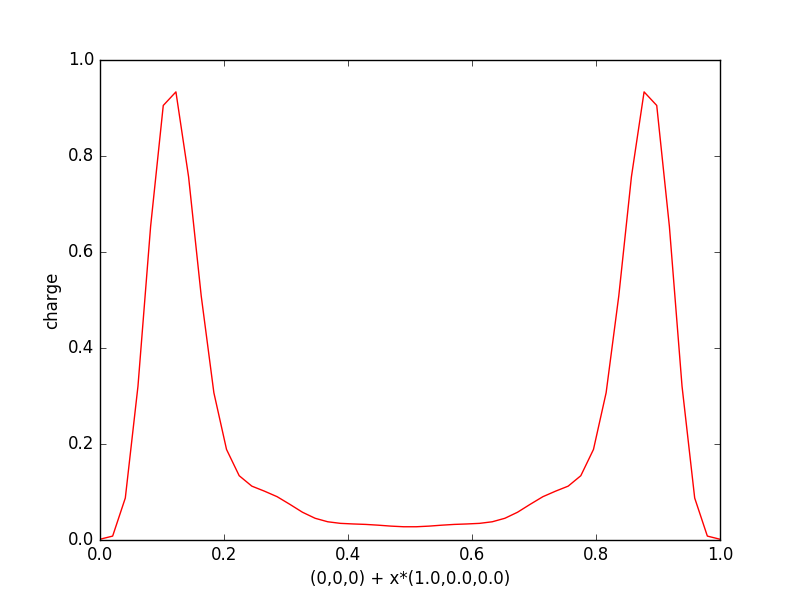
\includegraphics{{../examples/example2/figure_1}.png}


\section{Plotting a 2D section of the charge density  (examples 2)}
\label{tutorial:plotting-a-2d-section-of-the-charge-density-examples-2}
This example is similar to the previous one except for producing a 2D plot of a planar section of the electronic charge density. The plane is defined
by an initial point and two 3D vectors which define the plane.

\begin{Verbatim}[commandchars=\\\{\}]
\PYG{k+kn}{from} \PYG{n+nn}{postqe} \PYG{k+kn}{import} \PYG{n}{plot\PYGZus{}charge2D}

\PYG{n}{fin} \PYG{o}{=} \PYG{l+s+s2}{\PYGZdq{}}\PYG{l+s+s2}{./Ni.xml}\PYG{l+s+s2}{\PYGZdq{}}  				\PYG{c+c1}{\PYGZsh{} file xml produce by QE}
\PYG{n}{plot\PYGZus{}charge2D}\PYG{p}{(}\PYG{n}{fin}\PYG{p}{)}    			\PYG{c+c1}{\PYGZsh{} plot a 1D section of the charge }
                                	    
\PYG{c+c1}{\PYGZsh{}fig1 = plot\PYGZus{}EV(V,E,a)                  	\PYGZsh{} plot the E(V) data and the fitting line}
\PYG{c+c1}{\PYGZsh{}fig1.savefig(\PYGZdq{}figure\PYGZus{}1.png\PYGZdq{})}

\end{Verbatim}

As in the previous example, it is essentially a call to a single function, which is in this case \code{plot\_charge1D()}.
The output figure is:

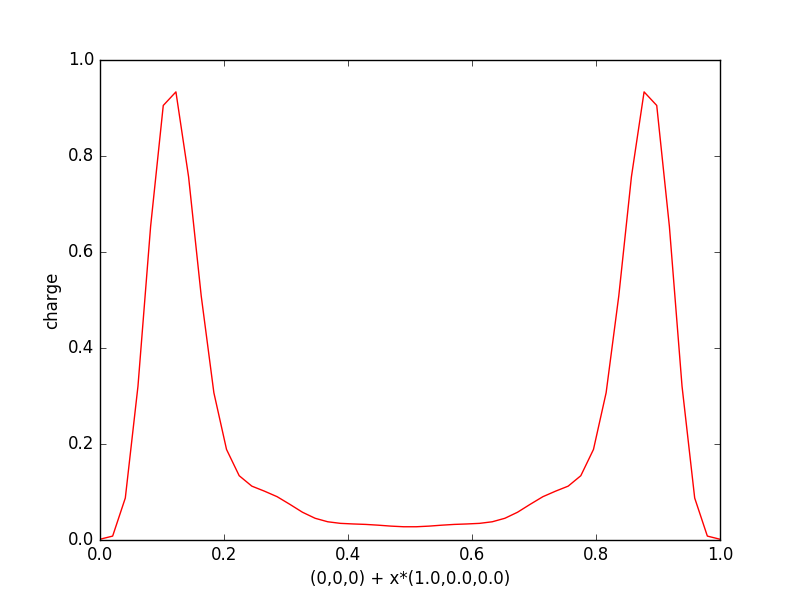
\includegraphics{{../examples/example2/figure_1}.png}


\section{Fitting the total energy using Murnaghan EOS (examples 3)}
\label{tutorial:fitting-the-total-energy-using-murnaghan-eos-examples-3}
The simplest task you can do with \code{postqe} is to fit the total energy as a function of volume \(E_{tot}(V)\) (example3). You can use
an equation of state (EOS) such as Murnaghan's or similar.  Currently the Murnaghan EOS and quadratic and quartic polynomials are implemented in \code{postqe}.

Let's see how to fit \(E_{tot}(V)\). This is the case of isotropic cubic systems (simple cubic, body centered cubic, face centered cubic) or systems which can be approximated as isotropic (for example an hexagonal system with nearly constant \(c/a\) ratio).

\begin{Verbatim}[commandchars=\\\{\}]

\PYG{k+kn}{from} \PYG{n+nn}{postqe} \PYG{k+kn}{import} \PYG{n}{fitEtotV}\PYG{p}{,} \PYG{n}{plot\PYGZus{}EV}

\PYG{n}{fin} \PYG{o}{=} \PYG{l+s+s2}{\PYGZdq{}}\PYG{l+s+s2}{./EtotV.dat}\PYG{l+s+s2}{\PYGZdq{}}  		\PYG{c+c1}{\PYGZsh{} file with the total energy data E(V)}
\PYG{n}{V}\PYG{p}{,} \PYG{n}{E}\PYG{p}{,} \PYG{n}{a}\PYG{p}{,} \PYG{n}{chi2} \PYG{o}{=} \PYG{n}{fitEtotV}\PYG{p}{(}\PYG{n}{fin}\PYG{p}{)}    	\PYG{c+c1}{\PYGZsh{} fits the E(V) data, returns the coefficients a and}
                                	\PYG{c+c1}{\PYGZsh{} the chi squared chi2}

\PYG{n}{fig1} \PYG{o}{=} \PYG{n}{plot\PYGZus{}EV}\PYG{p}{(}\PYG{n}{V}\PYG{p}{,}\PYG{n}{E}\PYG{p}{,}\PYG{n}{a}\PYG{p}{)}                  	\PYG{c+c1}{\PYGZsh{} plot the E(V) data and the fitting line}
\PYG{n}{fig1}\PYG{o}{.}\PYG{n}{savefig}\PYG{p}{(}\PYG{l+s+s2}{\PYGZdq{}}\PYG{l+s+s2}{figure\PYGZus{}1.png}\PYG{l+s+s2}{\PYGZdq{}}\PYG{p}{)}

\end{Verbatim}

The \code{fitEtotV()} needs in input a file with two columns: the first with the volumes (in \(a.u.^3\)), the second with energies (in \(Ryd/cell\)). It returns the volumes \emph{V} and energies \emph{E} from the input file plus the fitting coefficients \emph{a} and the \(\chi^2\) \emph{chi}. The fitting results are also written in details on the \emph{stdout}:

\begin{Verbatim}[commandchars=\\\{\}]
\PYGZsh{} Murnaghan EOS 		 chi squared= 6.3052908120e\PYGZhy{}09
\PYGZsh{} Etotmin= \PYGZhy{}1.6668753461e+03 Ry	 Vmin= 1.9256068649e+02 a.u.\PYGZca{}3	 B0= 3.9507640525e+03 kbar	 dB0/dV= 4.7877558697e+00
\PYGZsh{}\PYGZsh{}\PYGZsh{}\PYGZsh{}\PYGZsh{}\PYGZsh{}\PYGZsh{}\PYGZsh{}\PYGZsh{}\PYGZsh{}\PYGZsh{}\PYGZsh{}\PYGZsh{}\PYGZsh{}\PYGZsh{}\PYGZsh{}\PYGZsh{}\PYGZsh{}\PYGZsh{}\PYGZsh{}\PYGZsh{}\PYGZsh{}\PYGZsh{}\PYGZsh{}\PYGZsh{}\PYGZsh{}\PYGZsh{}\PYGZsh{}\PYGZsh{}\PYGZsh{}\PYGZsh{}\PYGZsh{}\PYGZsh{}\PYGZsh{}\PYGZsh{}\PYGZsh{}\PYGZsh{}\PYGZsh{}\PYGZsh{}\PYGZsh{}\PYGZsh{}\PYGZsh{}\PYGZsh{}\PYGZsh{}\PYGZsh{}\PYGZsh{}\PYGZsh{}\PYGZsh{}\PYGZsh{}\PYGZsh{}\PYGZsh{}\PYGZsh{}\PYGZsh{}\PYGZsh{}\PYGZsh{}\PYGZsh{}\PYGZsh{}\PYGZsh{}\PYGZsh{}\PYGZsh{}\PYGZsh{}\PYGZsh{}\PYGZsh{}\PYGZsh{}\PYGZsh{}\PYGZsh{}\PYGZsh{}\PYGZsh{}\PYGZsh{}\PYGZsh{}\PYGZsh{}\PYGZsh{}\PYGZsh{}\PYGZsh{}\PYGZsh{}\PYGZsh{}\PYGZsh{}\PYGZsh{}\PYGZsh{}\PYGZsh{}
\PYGZsh{} V *a.u.\PYGZca{}3) 		 Etot  (Ry)		 Etotfit  (Ry)		 Etot\PYGZhy{}Etotfit (Ry)	P (kbar)
1.7119697047e+02 	 \PYGZhy{}1.6668351807e+03	 \PYGZhy{}1.6668351587e+03	 \PYGZhy{}2.1971172146e\PYGZhy{}05	 6.2381531911e+02
1.7637989181e+02 	 \PYGZhy{}1.6668536038e+03	 \PYGZhy{}1.6668536431e+03	 3.9227047637e\PYGZhy{}05	 4.3099793531e+02
1.8166637877e+02 	 \PYGZhy{}1.6668660570e+03	 \PYGZhy{}1.6668660709e+03	 1.3986418708e\PYGZhy{}05	 2.6537059196e+02
1.8705745588e+02 	 \PYGZhy{}1.6668731355e+03	 \PYGZhy{}1.6668731117e+03	 \PYGZhy{}2.3822185085e\PYGZhy{}05	 1.2288704542e+02
1.9255414767e+02 	 \PYGZhy{}1.6668753764e+03	 \PYGZhy{}1.6668753461e+03	 \PYGZhy{}3.0392647432e\PYGZhy{}05	 1.3417016197e\PYGZhy{}01
1.9815747866e+02 	 \PYGZhy{}1.6668732871e+03	 \PYGZhy{}1.6668732784e+03	 \PYGZhy{}8.7825126229e\PYGZhy{}06	 \PYGZhy{}1.0577186614e+02
2.0386847338e+02 	 \PYGZhy{}1.6668673220e+03	 \PYGZhy{}1.6668673472e+03	 2.5205460133e\PYGZhy{}05	 \PYGZhy{}1.9727163448e+02
2.0968815635e+02 	 \PYGZhy{}1.6668579007e+03	 \PYGZhy{}1.6668579345e+03	 3.3793803595e\PYGZhy{}05	 \PYGZhy{}2.7643386187e+02
2.1561755211e+02 	 \PYGZhy{}1.6668454001e+03	 \PYGZhy{}1.6668453729e+03	 \PYGZhy{}2.7248831202e\PYGZhy{}05	 \PYGZhy{}3.4501482193e+02
\end{Verbatim}

Optionally, you can plot the results with the \code{plot\_EV()}. The original data are represented as points. If \emph{a!=None}, a line with the fitting EOS will also be plotted. The output plot looks like the following:

\includegraphics{{figure_1}.png}


\chapter{postqe package}
\label{postqe::doc}\label{postqe:postqe-package}

\section{Submodules}
\label{postqe:submodules}
Additional functions are available as submodules. Please note the documentation of these functions is still ongoing and can be incomplete or wrong.


\section{postqe.constants module}
\label{postqe:postqe-constants-module}

\section{postqe.eos module}
\label{postqe:postqe-eos-module}

\section{postqe.plot module}
\label{postqe:postqe-plot-module}

\section{postqe.readutils module}
\label{postqe:postqe-readutils-module}

\chapter{Indices and tables}
\label{index:indices-and-tables}\begin{itemize}
\item {} 
\DUspan{xref,std,std-ref}{genindex}

\item {} 
\DUspan{xref,std,std-ref}{modindex}

\item {} 
\DUspan{xref,std,std-ref}{search}

\end{itemize}



\renewcommand{\indexname}{Index}
\printindex
\end{document}
